\usetikzlibrary{calc}
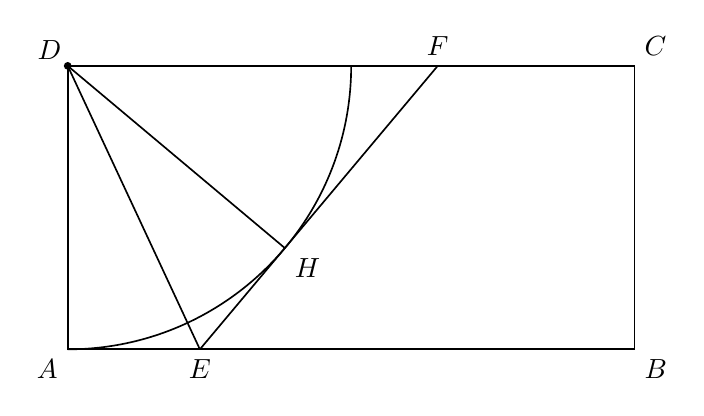
\begin{tikzpicture}[x=1cm,y=1cm,line width=.6pt,font=\normalsize]
\coordinate (A) at (0,0);
\coordinate (B) at (7.2,0);
\coordinate (C) at (7.2,3.6);
\coordinate (D) at (0,3.6);
\coordinate (E) at (1.6787,0);
\coordinate (H) at (2.7578,1.286);
\coordinate (F) at (4.6995,3.6);
\coordinate (T) at (3.6,3.6);
\draw (A)--(B)--(C)--(D)--cycle;
\draw (D)--(E);
\draw (D)--(H);
\draw (E)--(F);
\draw (A) arc[start angle=-90,end angle=0,radius=3.6cm];
\node[below left] at (A) {$A$};
\node[below right] at (B) {$B$};
\node[above right] at (C) {$C$};
\node[above left=2pt,inner sep=0pt] at (D) {$D$};
\node[below] at (E) {$E$};
\node[above] at (F) {$F$};
\node[below right] at (H) {$H$};
\fill (D) circle[radius=1.4pt];
\end{tikzpicture}
